% !TEX root =  manual.tex
\section{Markov Chain Monte Carlo}\label{sec:mcmc}

\subsection{Generating a trace}\label{subsec:GeneratingTheTrace}

After the emulator has been tuned, you can start to generate traces from it. A trace is a sequence of samples drawn from an emulator by a sampling algorithm. The command to generate a trace is

\commandline{madai\_generate\_trace stat1 trace.csv}

This command reads in the files stored in \path{stat1}, runs a Markov Chain Monte Carlo (MCMC) algorithm to explore the high-dimensional model parameter space, and produces a file named \path{trace.csv} in comma-separated value format (CSV). The \path{trace.csv} file is saved to the directory \\\path{stat1/trace/trace.csv}.

Each line of the CSV file contains information from one sample generated by the MCMC algorithm. The first entries in the line are the parameter in the model parameter space. The next entries in the line are the model outputs produced by running the model at that point in parameter space. The last entry is the log-likelihood that indicates how well the model outputs match the experimental data.

A brief sample from a CSV file created by \path{madai_generate_trace}  is shown below:

\begin{verbatim}
"p1","p2","p3","o1","o2","o3","o4","LogLikelihood"
1.19431,3.81693,0.604379,0.752093,3.88979,1.09151,0.907032,-1.44567
1.18372,3.8114,0.600692,0.747385,3.88466,1.08613,0.902906,-1.4521
1.17554,3.78698,0.610058,0.74376,3.86122,1.09977,0.899749,-1.46829
1.16455,3.77324,0.600326,0.738865,3.8481,1.08558,0.895453,-1.48468
1.17112,3.77779,0.592067,0.741777,3.85229,1.07355,0.897992,-1.51059
1.15852,3.78186,0.582758,0.736163,3.85649,1.05998,0.893065,-1.589
\end{verbatim}

The MCMC trace is stored as a csv file, \path{stat1/trace/trace.csv}. Each line describes the points in parameter space, $x_1\cdots x_P$, the observable values $y_1\cdots y_M$, and the log-likelihood. A header line at the beginning of the file lists the names of the parameters and observables.

\subsection{Analyzing the trace}\label{subsec:AnalyzingTheTrace}

Basic features of the trace can be extracted by invoking the command

\commandline{madai\_analyze\_trace stat1 trace.csv}

The command calculates several properties of the trace and writes them to the standard output:
\begin{itemize}\itemsep=0pt
\item the average and standard deviation for each parameter (integrated over all values of the other parameters), $\bar{x},\langle(x_i-\bar{x}_i)^2\rangle^{1/2}$, and $\langle(x_i-\bar{x}_i)^2\rangle^{1/2}/R_i$.
Here $R_i$ is the standard deviation of the prior distribution, so a value of unity shows that no discrimination of the parameters has been achieved.
\item the parameter values from the point in the trace with the highest likelihood.
\item a covariance matrix $\langle (x_i-\bar{x}_i)(x_j-\bar{x}_j)\rangle$.
\item a scaled covariance matrix $\langle (x_i-\bar{x}_i)(x_j-\bar{x}_j)\rangle/(R_iR_j)$.
\end{itemize}

An example output from \path{madai_analyze_trace}:
\begin{verbatim}
      parameter       average      std.dev.   scaled dev.    best value
            p0       11.9617      0.890389      0.220314         12.48
            p1       85.7203       7.04999      0.218052       93.2474
            p2     0.0847453     0.0404881      0.701274     0.0961365

best log likelihood
      -4.95619

covariance:
                          p0            p1            p2
            p0      0.792792       1.14868     0.0279174
            p1       1.14868       49.7023    -0.0634834
            p2     0.0279174    -0.0634834    0.00163929

scaled covariance:
                          p0            p1            p2
            p0     0.0485383    0.00879092      0.119646
            p1    0.00879092     0.0475469    -0.0340089
            p2      0.119646    -0.0340089      0.491786
\end{verbatim}

 \subsection{Posterior Sampling}\label{subsec:PosteriorSampling}

 It is often useful to view a sampling of points
 representative of the posterior distribution. Such a
 sampling can be generated by the command

 \commandline{madai\_generate\_posterior\_samples stat1 trace.csv 20}

The third argument specifies how many samples will be drawn from the file \path{trace.csv}. These points will be written to files in a directory specified by the POSTERIOR\_ANALYSIS\_DIRECTORY. If this setting is not specified, the files will be placed in \path{stat1/posterior_model_output}. The files and directories generated by this program are in the same format as used for the
 parameter files in the \path{model_output} directories. For
 example, if there are 20 points the parameters will be
 stored in the files

\path{stat1/posterior_model_output/run0000/parameters.dat}\\
$\vdots$\\
\path{stat1/posterior_model_output/run0019/parameters.dat}.

 The points are chosen to be evenly spaced from the MCMC
 trace. In addition to the \path{parameters.dat} files, the
 command also writes a file
 \path{stat1/posterior_model_output/runXXXX/trace_results.dat} where \path{XXXX} is a zero-padded index of the run. This
 file contains the observables $y_1\cdots y_M$ and the
 log-likelihood as written in the CSV file.

 Once the sampling of points are generated from the
 continuum, the user can use them to run the full model and
 see whether the resulting model output indeed matches the
 experimental measurements. Additionally, the user can then
 compare the observables from the full model runs to those
 from the emulator, i.e., those taken from the csv file in
 the trace and stored in
 \path{stat1/posterior_model_output/run$n$/trace_results.dat}.

\subsection{Publication Quality Plots of the Posterior Distribution}\label{subsec:PublicationQualityPlots}

One useful representation of the trace is that of one- or two-dimensional projections of the posterior distribution. Simply stated, these plots represent the probability of either a single parameter integrated over all values of the remaining parameters, or of two parameters integrated over the remaining $P-2$ parameters. These distributions are easily extracted from the csv file by making a distribution of the sampling points binned by a single parameter $x_i$ or of a pair of parameters $x_i$ and $x_j$.

\path{madai_gnuplot_scatterplot_matrix}
creates a $P\times P$ matrix of scatterplots as exemplified in Fig. \ref{fig:scatterplot}. The off-diagonal plots represent two-dimensional projections of the posterior distribution, while the diagonal plots show one-dimensional projections. 

This program depends on Python  (version 2.4 or later) and on gnuplot (version 4.4 or later).

\commandline{madai\_gnuplot\_scatterplot\_matrix} {\it input.csv} {\it output.pdf} {\it parameter\_description\_filename} $N_{\rm bins}$

To use the \path{madai_gnuplot_scatterplot_matrix}, first verify that \path{gnuplot} is installed and located in the user's \path{PATH}.  Otherwise, the path of the gnuplot executable can be specified with the \path{GNUPLOT_COMMAND} environment variable.

Next, create the file file \path{parameter_description.dat}, which is similar in format to \path{parameter_priors.dat}. It lists the range of the parameters to be plotted and the variable names which will label the axes. For example, a file with graph with three parameters could be:
\begin{quote}
\begin{verbatim}
UNIFORM X0   -2.0  2.0    X_0 (cm)
UNIFORM K     0.5  4.0    K (ergs/cm^2)
UNIFORM TEMP  0.5  10.0   T (deg.)
\end{verbatim}
\end{quote}
The first four columns are identical to what is found in \path{parameter_priors.dat} file, but everything past the last column describes the axis label. The variable names in the second column need to match the names in the header line of the CSV file describing the trace. The axis labels can be written in the format gnuplot uses for labels. For instance, the character $\alpha$ can be accessed as \texttt{\{/Symbol a\}}. A subset of the parameters can be chosen by commenting out the line with \path{#}. The ranges for the plots can also be chosen to differ from what is in the prior. The command might look like

\begin{quote}
\texttt{
\commandprompt{}madai\_gnuplot\_scatterplot\_matrix \continueline
    stat1/trace/trace.csv \continueline
    stat1/fig/scatterplot.pdf \continueline
    stat1/parameter\_description.dat \continueline
    50}
\end{quote}

The density plots would have a resolution of 50$\times$50. The command will produce temporary files which will be stored in a temporary directory in an OS-specific location.  In the temporary directory is a \path{scatterplot_matrix.gplt} gnuplot script. One can now regenerate the pdf file by editing the gnuplot script and re-executing it:

\begin{figure}
\begin{center}
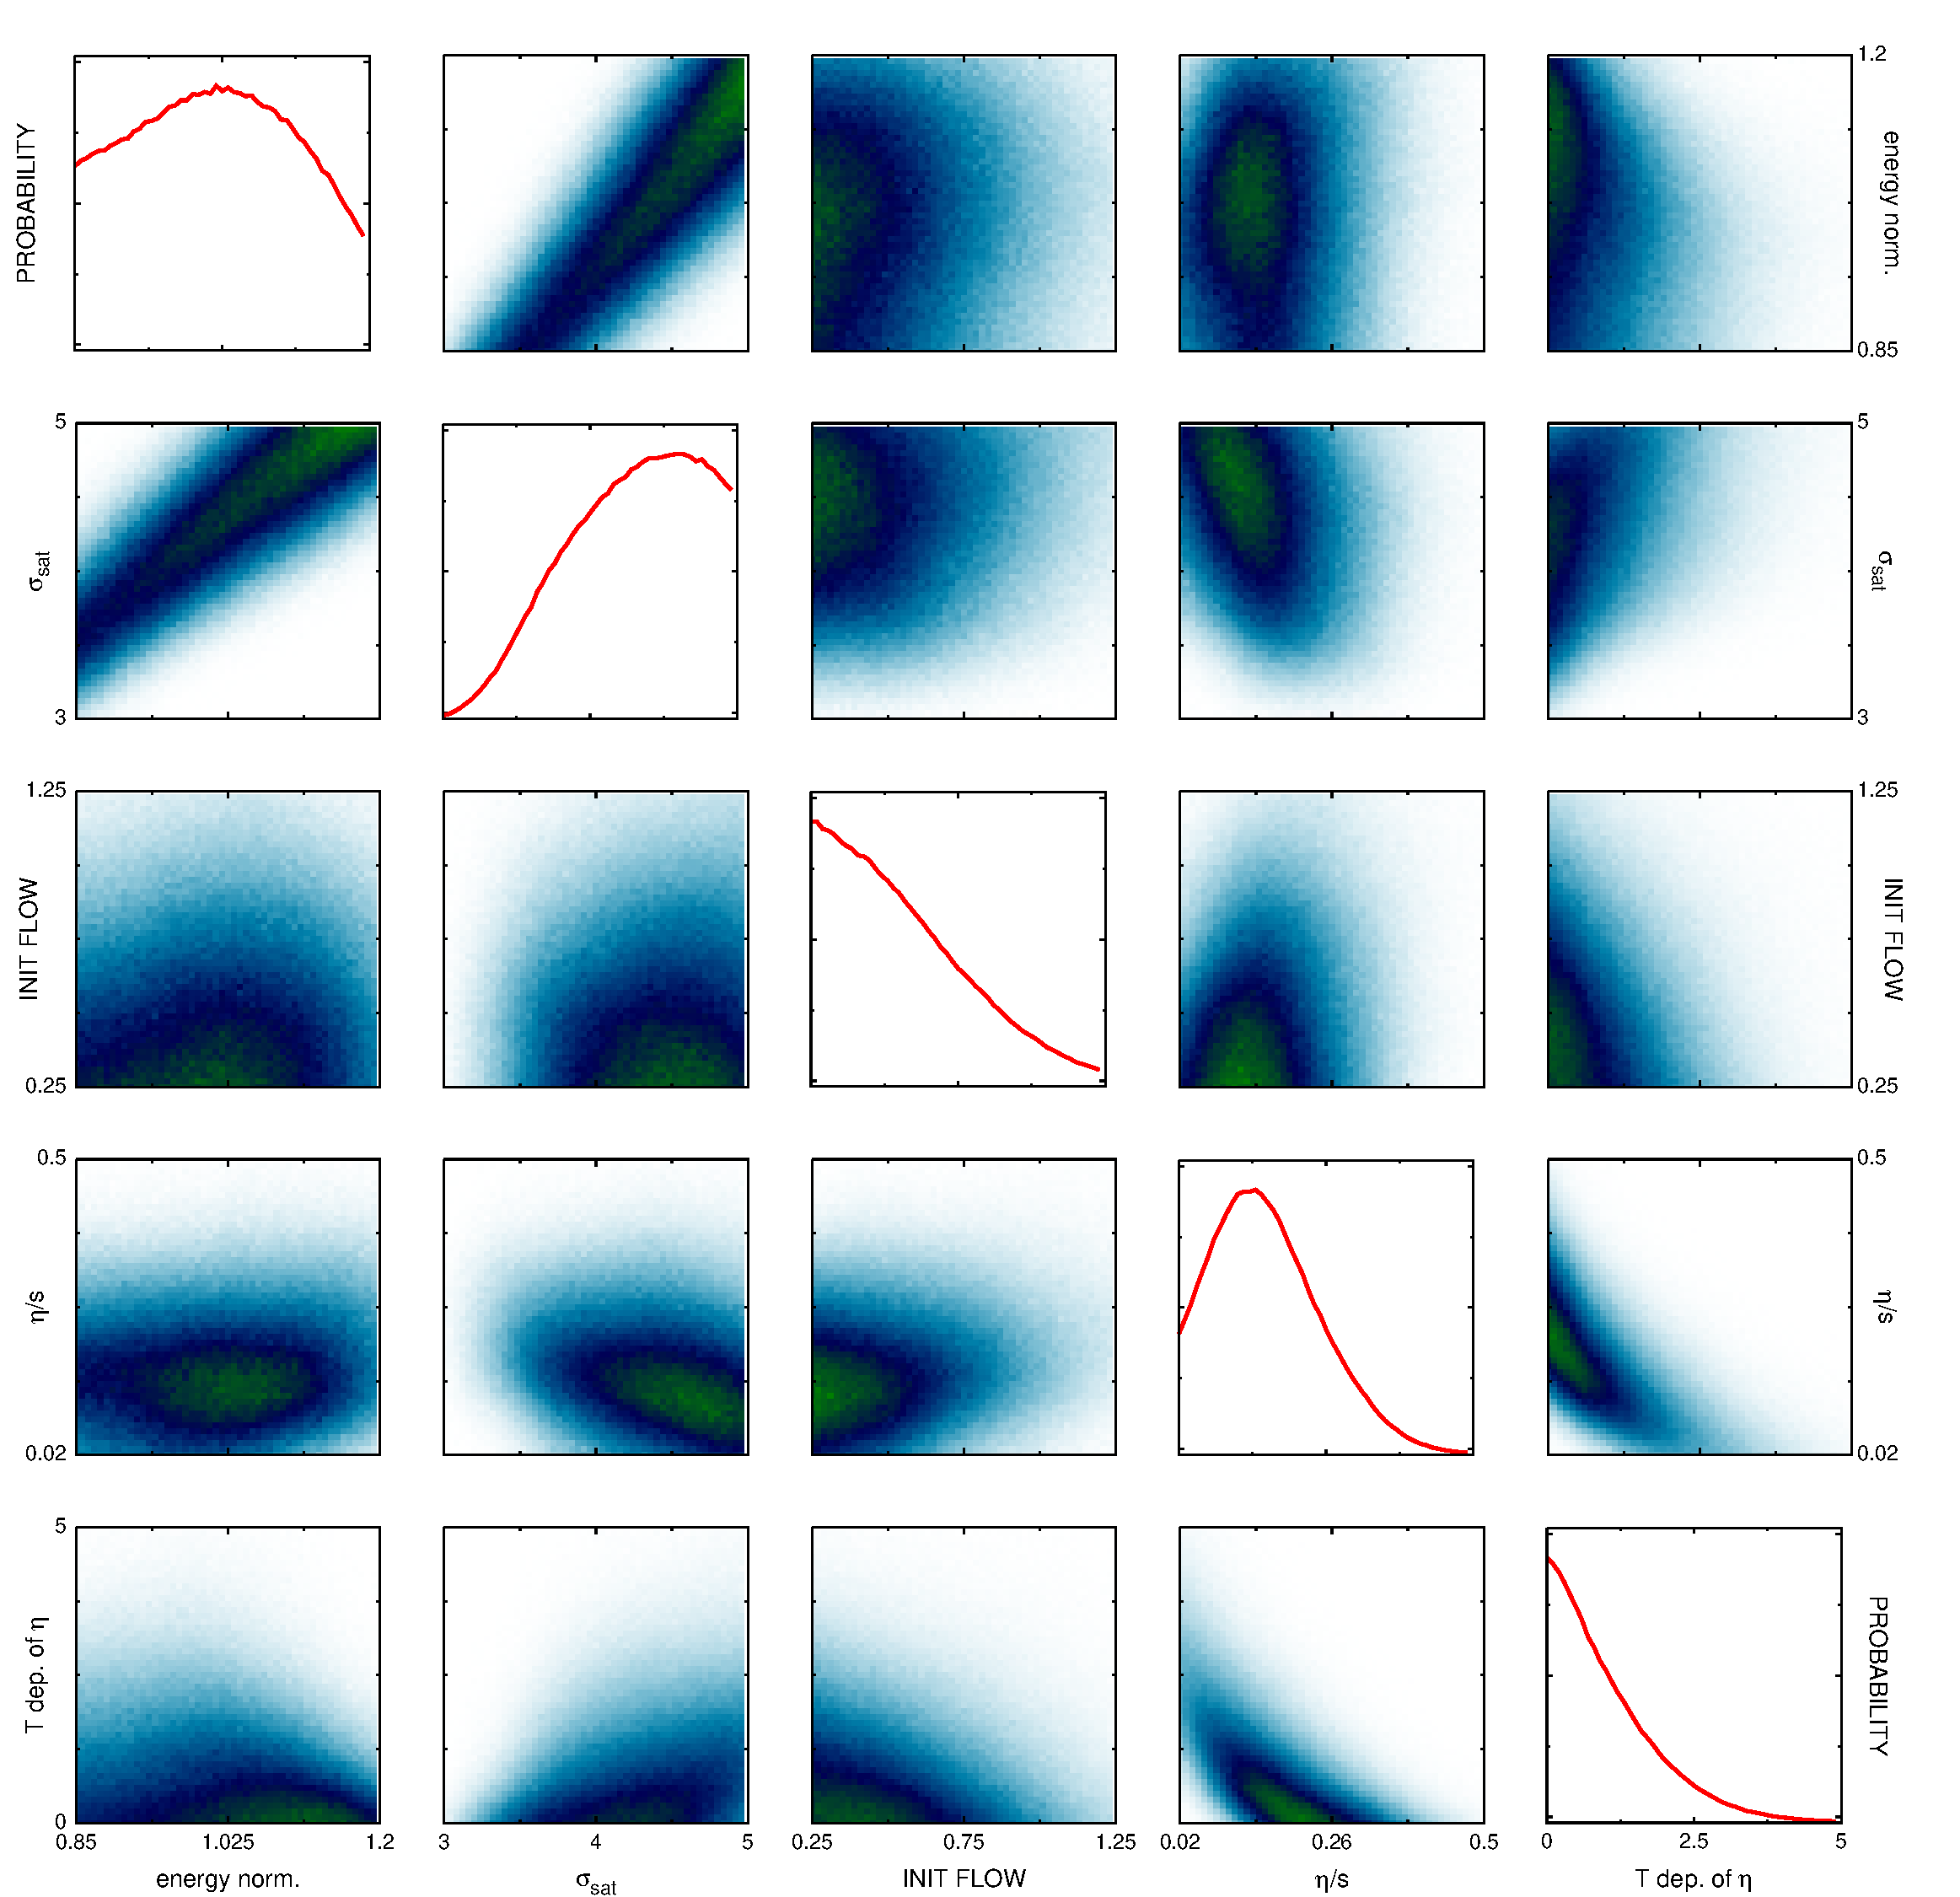
\includegraphics[width=0.8\textwidth]{figs/rhic.pdf}
\end{center}
\caption{\label{fig:scatterplot}
A Scatterplot Matrix }
\end{figure}



%%  LocalWords:  gnuplot Scatterplot LocalWords
